\section{Formulation and Proposed Algorithm}

\subsection{Problem Formulation}
\label{sec::ProblemFormulation}


%\begin{figure}
%\begin{center}
%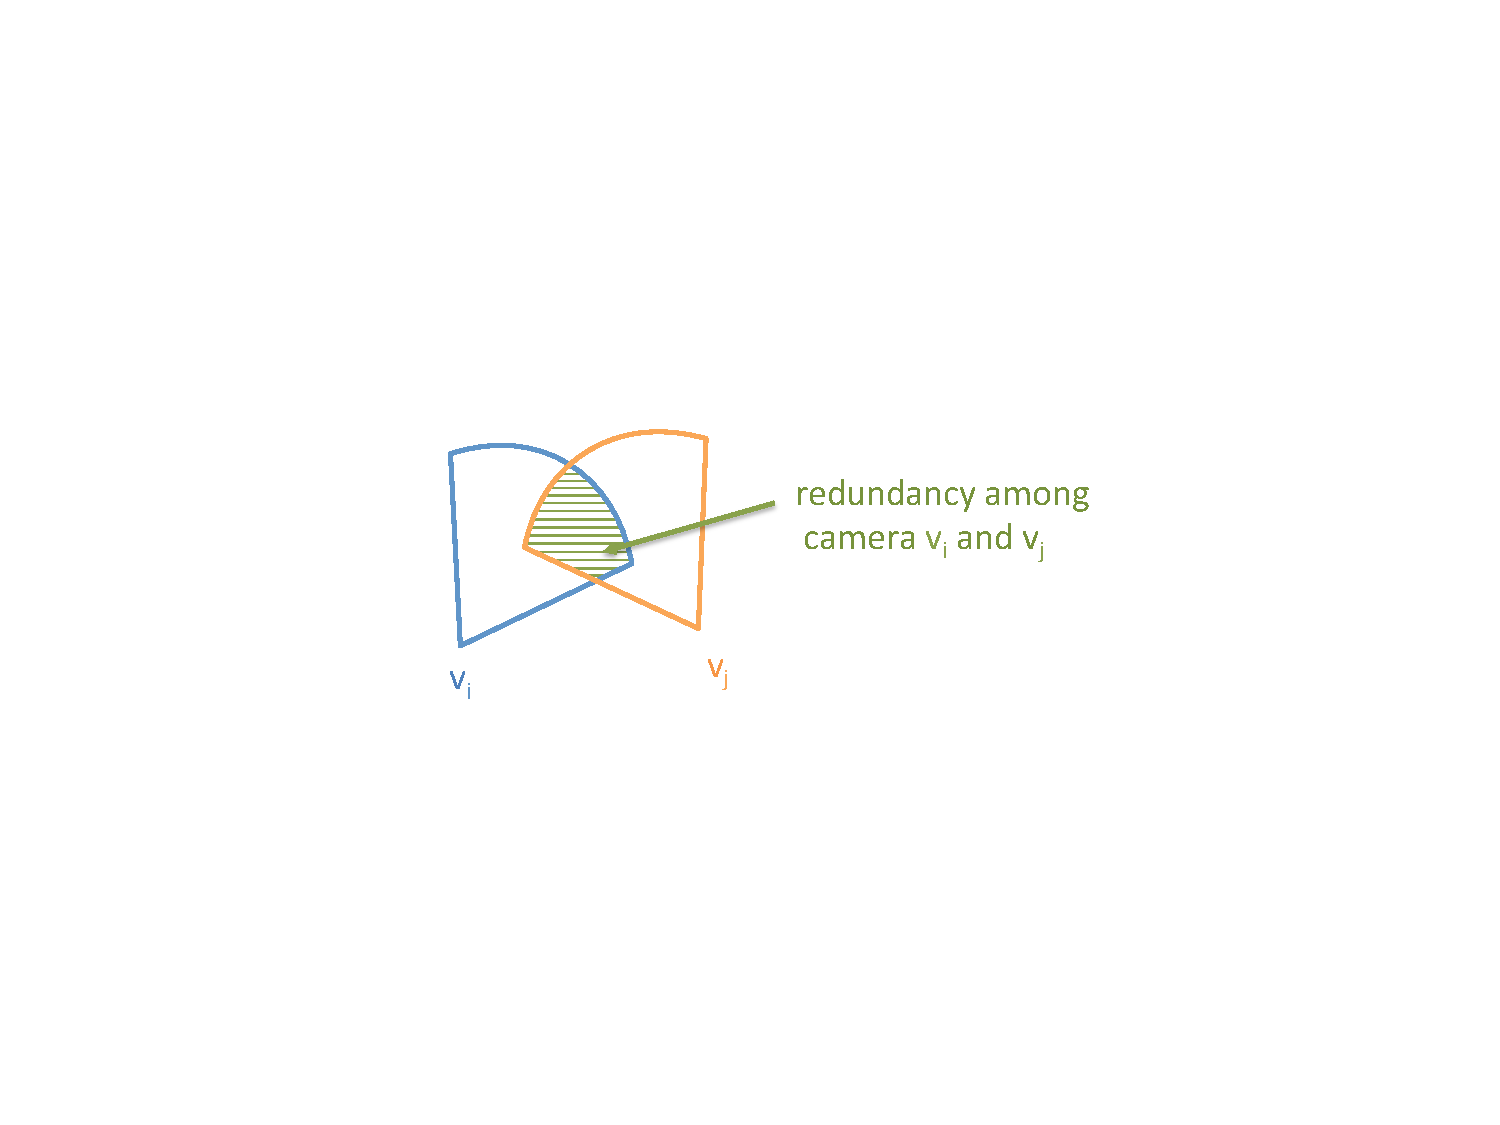
\includegraphics[width=0.7 \columnwidth]{./fig/cameraRedundancy.pdf}
%\caption{\label{fig::cameraRedundancy}Redundancy among cameras}
%\end{center}
%\end{figure}

\ignore{
As we mentioned before, our purpose in this paper is to minimize the total
encoded bits for transmission of a wireless multimedia sensor network.
Given a set ${V=\{v_1,v_2, \cdots v_N \}}$ of cameras placed in a wireless
multimedia sensor network, where each camera $v_i$ produces image $X_i$.
If these cameras are deployed under a dense scenario, there might be some
redundancy among the cameras in $V$.
As Figure~\ref{fig::cameraRedundancy} shows, if two camera $v_i$ and $v_j$ are
installed at a neighboring position and both have the same area of interest,
there might have some overlap among their collected scene.
Therefore, if we serve the network in an independent way (all cameras in $V$
encode its data independently), we might cause a waste of using the limited
radio resource since there is no need to transmit the redundant part.

Since we have mentioned that using a dependent encoding scheme is a more
efficient way to serve the wireless multimedia sensor network.
It rise a problem that how to reduce the transmission of the redundant part.
For the scenario in Figure~\ref{fig::cameraRedundancy}, we can either
compress image $X_i$ based on the prediction of $X_j$ or compress $X_j$ based
on the prediction of $X_i$.
Which mode to choose should depend on the scheduling sequence of cameras, since
a camera can only compress its data based on those previous scheduled cameras.
Therefore, in order to reduce the total required encoded bits of a network, we
will explore an algorithm to determine a proper schedule in the following
sections.
}

\ignore{
We consider a scenario where a set of cameras are deployed at different locations
to collect snapshot views and transmit back to the aggregator (collector) periodically.
%To simplify our problem, we assume in this paper that all the cameras in $V$
%need to encode its collected image and transmit to an aggregator.
Since subsets of cameras may be deployed at nearby locations for providing different
perspectives of views, images collected by individual cameras may exhibit correlation.
If a camera can overhear transmissions from nearby cameras, it can perform
{\em overheard source coding} to reduce the amount of bits required to encode
its image.
%Besides, we also assume that all cameras in $V$ can perform an overhearing
%source coding scheme.
Specifically, the camera
%That is, they are able to gather others transmission and use the gathered image
can reference the image overheard from nearby camera
for motion prediction. If the reference image is highly correlated with the target
image, the compression ratio will be high.
% so that the encoded bits can be reduced.
%
In the target scenario, since a camera can overhear only nearby cameras scheduled 
before it, the order of transmission (transmission schedule) plays an important role 
in determining
the efficiency for reducing the total amount of bits required for transmitting
all collected images.
%However, a camera $v_i$ can only overhears transmission from preceding cameras
%and the encoding efficiency would be decrease if the gathered image of those
%preceding cameras is not correlated to $v_i$.
%Therefore, our problem is to determine a transmission order so that most of the
%cameras in $V$ can reference from its most correlated frame.
}

Let ${V=\{v_1,v_2, \cdots v_N \}}$ be the set of $N$ cameras under consideration
and $X_i$ be the snapshot of image produced by camera $v_i$.
%Each camera $v_i$ produces a snapshot of image $X_i$.
%
Denote $H(X_i)$ as the amount of bits required to encode $X_i$ independently (entropy),
%We now assume that the entropy of independently encoding camera $v_i$ equals $H(X_{i})$,
and	$H(X_{i}|X_{j})$ as the amount of bits required if $X_j$ is used as
reference for encoding $X_i$ (conditional entropy).
%conditional entropy denotes the conditional entropy if camera
%$v_i$ reference from camera $v_j$ when encoding.
Clearly, for camera $v_i$ to reference the image captured by camera $v_j$, it is
required that $v_j$ is scheduled before $v_i$ and the transmission range of camera
$v_j$ covers camera $v_i$.
%One thing to mention is that if camera $v_i$ tends to reference from camera
%$v_j$, not only camera $v_j$ needs to be scheduled before $v_i$, but also the
%transmission range of camera $v_j$ must cover $v_i$.
Based on such a notation, the total amount of encoded bits for transmission can
be written as follows:
%
\begin{equation}
\sum_{i=1}^{N} \sum_{j=1}^{N} \alpha_{ij} H(X_i|X_j),
\label{eq::totalBits}
\end{equation}
%
where ${H(X_i|X_i) = H(X_i)}$ for sake of notation simplicity and
${\alpha_{ij} \in \{0,1\}}$ is an indicator variable such that
%where
${\alpha_{ij}=1}$ when camera $v_i$ overhears camera $v_j$ and
${\alpha_{ii}=1}$ when camera $v_i$ performs independent encoding.
%indicates that camera $v_i$ is independently encoded.
%
%Essentially, $H(X_i|X_i)$ will equals the size of H.264 header.
%For sake of notation simplicity, ${H(X_i|X_i) = H(X_i)}$ if camera $v_i$
%performs independent encoding without overhearing any other cameras.
%That is, if camera $v_i$ tends to overhear itself, then $v_i$ will encode
%independently.
%
We require that
\begin{equation}
\sum_{j=1}^{N} \alpha_{ij} = 1,\;\forall i \in V,
\label{eq::overNumConstraint}
\end{equation}
%
such that each camera in $V$ is allowed to overhear \emph{only one} camera
in its neighborhood.
%

\ignore{
Now the formulation of our problem becomes:
\begin{equation}
\text{minimize}~\sum_{i=1}^{N} \sum_{j=1}^{N} \alpha_{ij} H(X_i|X_j),
\label{eq::objective}
\end{equation}
subject to
\begin{align}
\sum_{j=1}^{N} \alpha_{ij} = 1,~&\forall i \in V,
\label{eq::overNumConstraint} \\
\tau_i - \tau_j \geq \alpha_{ij},~&\forall i,j \in V, i \neq j,
\label{eq::overTimeConstraint}
\end{align}
where constraint~\eqref{eq::overNumConstraint} means that each camera in $V$
must overhear and reference from \emph{only one} camera.
Constraint~\eqref{eq::overTimeConstraint} is for the transmission time
constraint in the overhearing encoding scheme.
We here denote the time slot allocated for camera $v_i$ as $\tau_i$ (if $v_i$
transmits at the first time slot then $\tau_i = 1$; if $v_i$ transmits at the
second time slot then $\tau_i = 2$; etc).
Therefore, if camera $v_i$ tends to overhear camera $v_j$, $v_j$ must be
transmitted before $v_i$ starts encoding, which would lead to the inequality of
constraint~\eqref{eq::overTimeConstraint}.
} 